\documentclass{article}
\usepackage[utf8]{inputenc}
\usepackage{graphicx}

\graphicspath{{./images/}}



\title{
    \vspace{-2cm}
    \Huge WRO 2025 \\ Future Engineers \\[0.5cm]
    \LARGE Team Carcharodontosaurus
}

\author{
    \large Sebastian Eggerer, Matthew Greiner, Norbert Niering \\ [0.2cm]
    \large Josef-Hofmiller Gymnasium
}

\date{}

\begin{document}

\maketitle
\begin{center}
  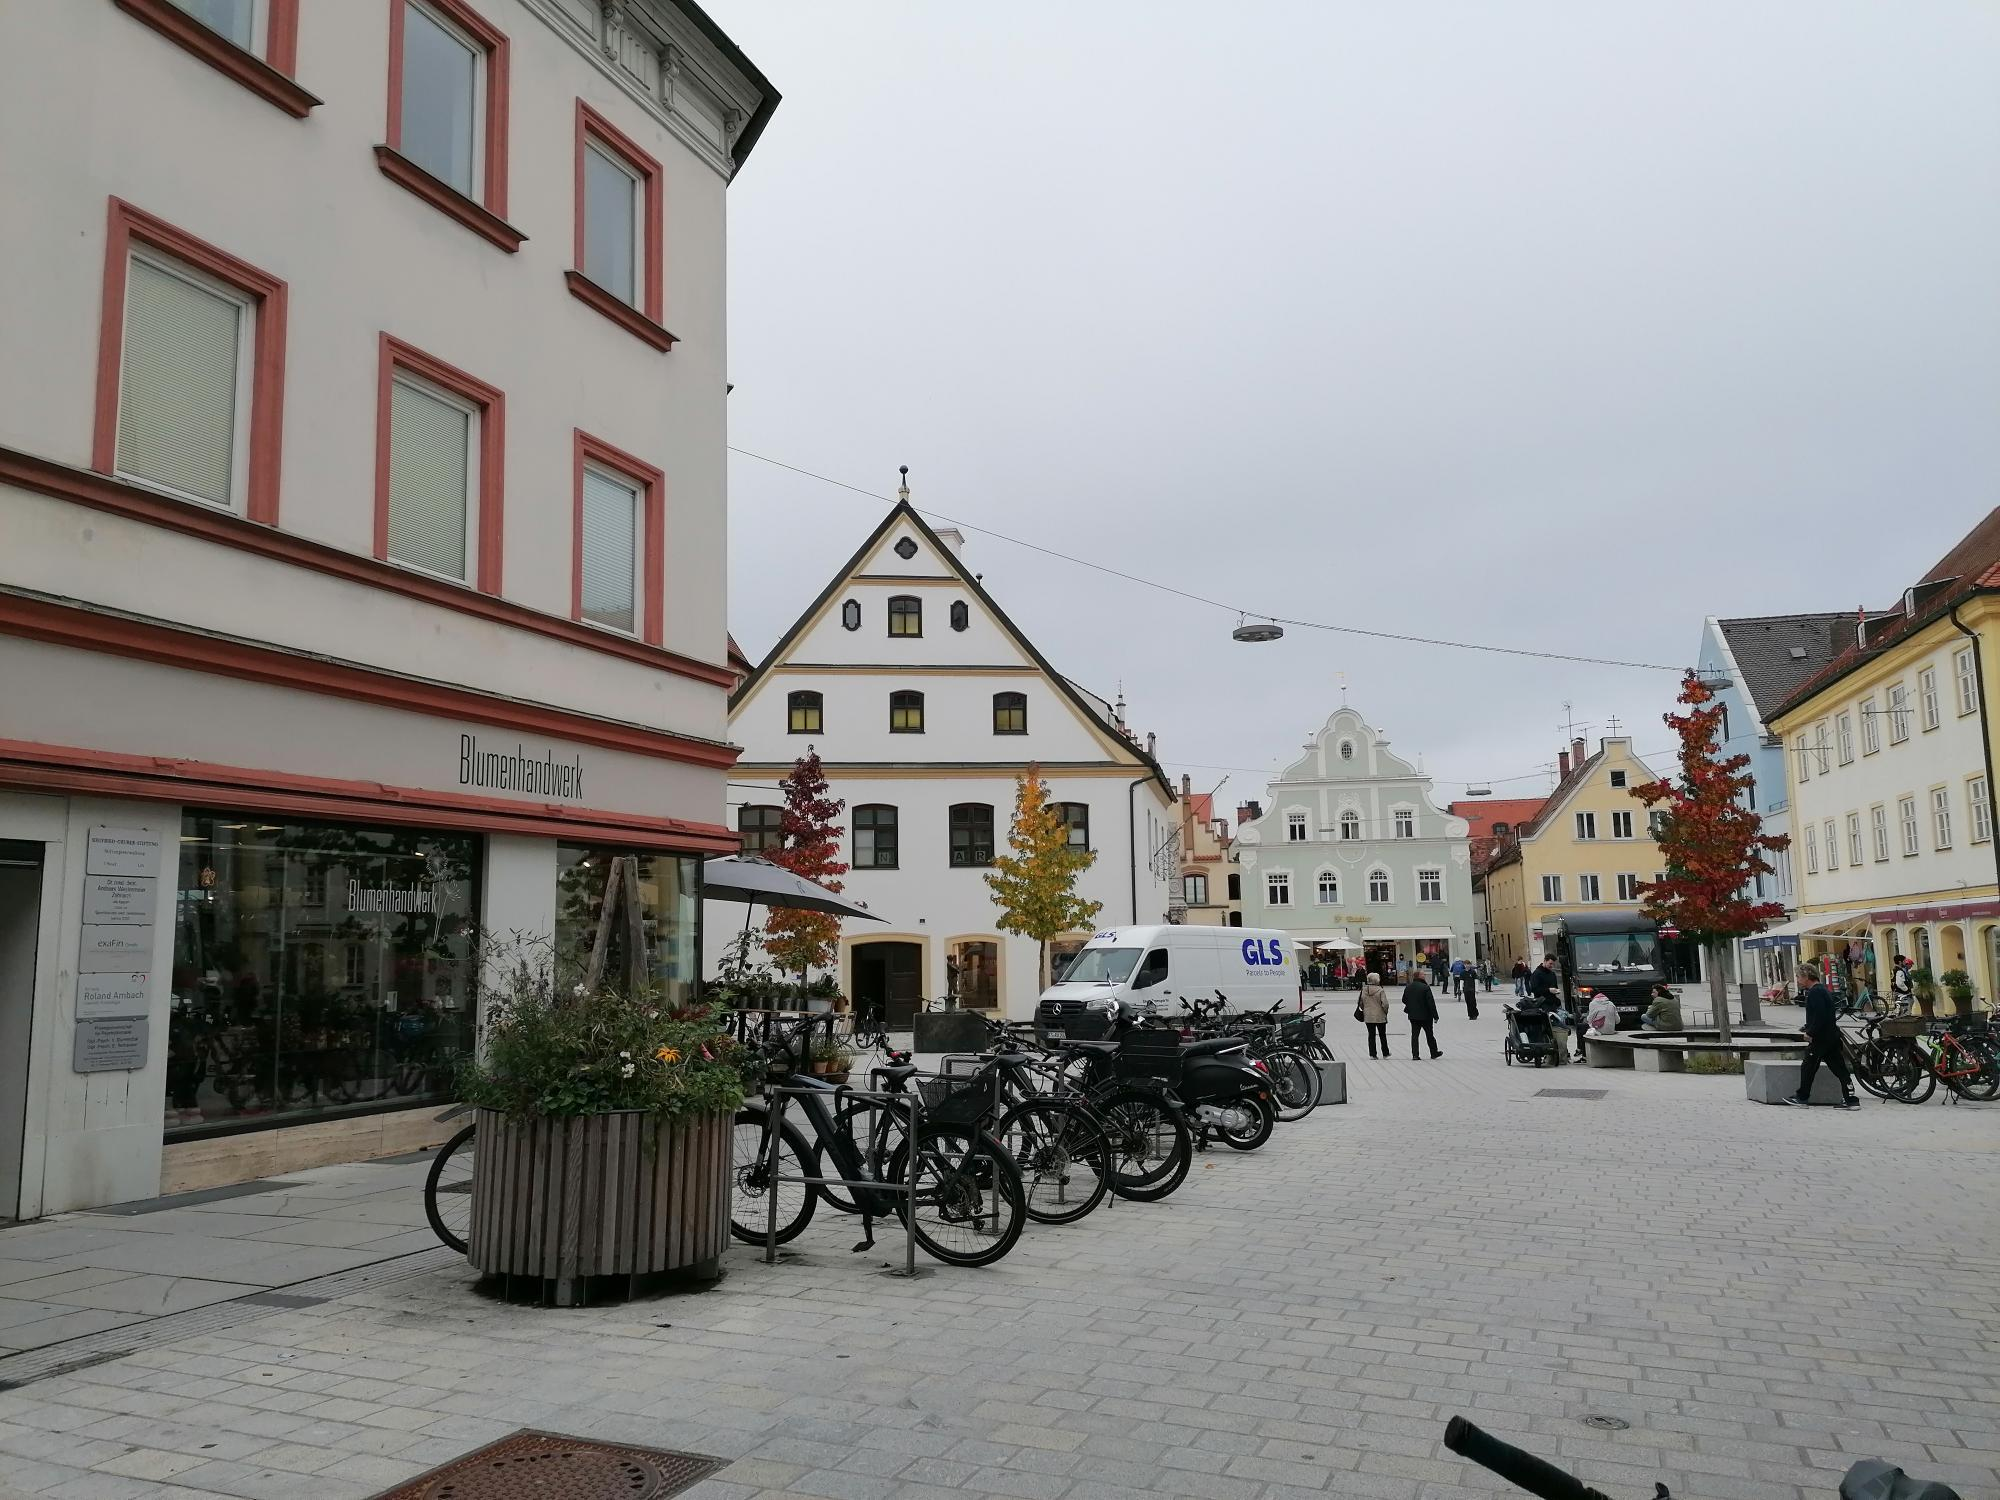
\includegraphics[scale=0.17]{team_photo}
\end{center}

% end of title page

\newpage

\section{Motoren}
Wir verwenden für unseren Roboter zwei Motoren, vorne befindet sich ein Lenkmotor und hinten ein Antriebsmotor.
Dieses System sorgt für Stabilität, der Roboter wird durch den Heckmotor, welcher über ein relativ hohes Gewicht verfügt,
gleichmäßig und ohne Taumeln beschleunigt, während der weit vorne angebrachte, sowie deutlich leichtere, Lenkmotor ein genaues Lenken ermöglicht.
Es handelt sich um einen klassischen Hinterradantrieb.\newline
Die Auswahl des Antriebmotors erschien zunächst als leicht. Wir entschieden uns dafür, einen bereits gebrauchten DC-Motor aus einem RC-Auto auszubauen und
diesen in unserem Roboter zu verwenden. Nach einigen Tests stellte sich jedoch heraus, dass dieser bei niedrigen Geschwindingkeiten nicht
die gewünschte Genauigkeit lieferte.\newline
In Folge dessen sahen wir uns gezwungen einen unseren Bedürfnissen angepassten Motor zu beschaffen.
Diesmal bestellten wir einen neuwertigen 6V DC-Motor, welcher die von uns gestellten Anforderungen erfüllte.
Mit einer Untersetzung von 18:1 bei einer Drehzahl von 6200U/min verfügte der Motor ebenfalls über ein für uns passendes Drehmoment.\newline
Beim Lenkmotor entschieden wir uns, einen Servo-Motor zu verwenden, da dieser über eine höhere Präzision verfügt und somit ein exaktes Lenken ermöglicht.
Servo-Motoren bieten den Vorteil, dass sie durch ihre integrierten Sensor zur Positionsbestimmung eine präzise Winkelpositionierung erlauben,
was für die Lenkung unseres Roboters essenziell ist. Nach mehreren Tests konnten wir feststellen,
dass der Servo-Motor nicht nur die gewünschte Genauigkeit liefert, sondern auch eine schnelle Reaktionszeit aufweist,
was besonders bei raschen Richtungswechseln entscheident ist.\newline
\begin{center}
  \includegraphics[scale=0.3]{motoren_position.png}
\end{center}
Zum Schutz sind beide Motoren in einem eigens 3D-gedruckten Gehäuse untergebracht,
welches speziell für die Anforderungen unserer Hardware entworfen wurde.
Dieses Gehäuse schützt die Motoren vor äußeren Einflüssen wie Staub und Stößen und sorgt gleichzeitig für eine stabile Befestigung am Chassis.

\section{Energie \& Sensoren}
Für das Bereitstellen von Strom verwenden wir einen 7,4V und 2,2Ah Lithium-Polymer Akku, welcher über ein relativ geringes Gewicht verfügt
und sich dadruch Ideal für unser Unterfangen eignet.\newline
Wir verwenden drei unterschiedliche Arten von Sensoren, um die Umgebung und Position des Roboters zu erkennen und daraus eindeutige Handlungsanweisungen
zu erstellen.\newline
Zur Erfassung der farbigen Quader, verwenden wir eine Kamera, diese erfasst laufend Daten über alles was vor dem Roboter liegt,
welche dann in unserem Programm ausgewertet werden, um die Position und Farbe der Quader zu bestimmen.
Die Kamera ist so positioniert, dass sie einen optimalen Blickwinkel auf das Spielfeld hat,
wodurch eine zuverlässige Erkennung gewährleistet wird.
Zudem ist das Kamerasystem von einem 3D-gedruckten Gehäuse umgeben.\newline
Der Roboter verfügt über vier Ultraschallsensoren, einen an jeder Seite, mit einem Erfassungswinkel von 15°
und einer Reichweite von bis zu 4,5m.
Diese werden für die Erfassung der Entfernung zu Hindernissen, wie etwa den Wänden, verwendet.
Alle Ultraschallsensoren sind ebenfalls durch ein Gehäuse geschützt.\newline
Der im Orientierungsmodul verbaute Gyrosensor, welcher die Orientierung und Drehbewegungen des Roboters misst,
erlaubt uns Drehungen und Bewegungen zu überprüfen und gegebenenfalls zu korrigieren.
Dies ist insbesondere bei längerem Betrieb wichtig.
\begin{center}
  \includegraphics[scale=0.3]{sensoren_position.png}
\end{center} 
Durch die Kombination dieser Sensoren ist unser Roboter in der Lage, seine Umgebung effektiv wahrzunehmen
und entsprechend darauf zu reagieren.

\section{Hindernisse}

\section{Fotos}

\section{Engineering \& Design}

\end{document}